\chapter{Implementation}

In this chapter, we delve into the practical aspects of creating \ac{AI} agents capable of tackling abstract strategy games. The focus is on constructing adaptable, game-agnostic systems that can be applied to a variety of games, ranging from the simplicity of Tic-tac-toe to the profound strategic depths of Go, with our primary case study being the game of Quoridor.

\ac{Csharp}, is selected as the language of choice, mainly for its robustness, versatility, and strong support for object-oriented programming paradigms. \ac{Csharp}'s rich feature set makes it an excellent tool for developing sophisticated \ac{AI} frameworks that require a blend of performance, maintainability and readability.

\section{Interfaces}

The architecture of our implementation leverages interfaces, fundamental constructs in object-oriented design that define contracts for implementing classes. These interfaces specify a set of methods related to game mechanics, which are vital for the operation of \ac{AI} agents. Through the use of generic parameters \textbf{TPlayer}, \textbf{TMove}, and \textbf{TGame}, these interfaces offer a framework that is adaptable to various game entities such as players, moves, and game states.

The fundamental interfaces and their contents include the following:

\begin{lstlisting}
interface IPlayer<TPlayer>
{
    /*
     *Retrieves the active player in the game.
     *Parametrized over TPlayer instance
     */
    TPlayer CurrentPlayer { get; }
}

interface IDeepCopy<T>
{
    /*
     *Create a deep copy of an instance, (e.g. of a game
     *state, allowing for safe simulations and backtracking)
     *without altering the actual object.
     */
    T DeepCopy();
}

interface IStaticEvaluation
{
    /*
     *Computes a heuristic evaluation of the current game state,
     *indicating the desirability of the state for the player who
     *is currently maximizing or minimizing the game value
    */
    public double Evaluate(bool currentMaximizer);
}



interface ITerminal
{
    /*
    * A property that checks whether the game has
    * reached a terminal state.
    */
    bool HasFinished { get; }
}

interface IValidMoves<TMove>
{
    /*
    *Returns all the valid moves that can
    *be made from the current state.
    */
    IEnumerable<TMove> GetValidMoves();
}

interface IOpponent<TPlayer>
{
    /*
    * Retrieves the active opponent in the game state,
    * parametrized over TPlayer
    */
    TPlayer Opponent { get; }
}

interface INeighbors<TMove>
{
    /*Yields the neighboring positions or states from a given
    *position pos, crucial for deter-mining potential player actions
    */
    IEnumerable<TMove> Neighbors(TMove pos);
}

interface IMove<TMove>
{
    // Applies a move to the game state
    void Move(TMove move);

    /*
    *Reverts a move, restoring the
    *game state to its previous condition
    */
    void UndoMove(TMove move);
}

interface IRandomizableMoves<TMove>
{
    /*
     *Returns all the valid moves (that guide the current game state
     *towards the terminal state) that can be made from the current
     *state and can be used by the random agent
    */
    public IEnumerable<TMove> RandomizableMoves();
}

\end{lstlisting}

They form the backbone of the implemented \ac{AI} system, ensuring that the agents are versatile and can be adapted to new games with minimal changes to the underlying codebase.

\section{Agents}

In this section, we discuss the generic \ac{AI} agent implementation, namely Random, Semi-Random, Minimax, A-Star, Monte Carlo Tree search, and describe how the aforementioned interfaces are used as building blocks for the algorithm.

\subsection{Random Agent}
We consider a random agent as a baseline for comparing the performance of the other implemented agents. 

The random agent uses the \textbf{IValidMoves\textless{}TMove\textgreater{}} interface to get a list of all valid moves, and then picks move at random. The pseudocode for the random agent along with the interface is given below:

\begin{lstlisting}
public class RandomStrategy<TMove, TGame, TPlayer>(int seed)
where TGame : IValidMoves<TMove>
{    
    public TMove BestMove(TGame game, TPlayer player)
    {
        // IValidMoves<TMove>
        var validMoves = game.GetValidMoves();

        //pick a random number corresponsing to the index of the move
        var randIndex = _random.Next(0, validMoves.Count());

        //return the random move
        return validMoves.ElementAt(randIndex)
    }
}
\end{lstlisting}

As described above, the Random Agent picks a move from the set of valid moves based on the \textbf{IValidMoves\textless{}TMove\textgreater{}} interface.

\subsection{Semi-Random agent}

There are cases where we want to return a random move, but we don't want the game to continue forever by the random agent possibly returning move that never end in a terminal state. In this case, we want to guide the random agent to produce a random move, but also make sure the game will terminate eventually. This algorithm is especially useful for the Simulation step of the \ac{MCTS} algorithm as an approach to shorten the game length to reach the terminal state.

For this purpose, we define the Semi-Random agent defined by the following code. 

\begin{lstlisting}
public class SemiRandomStrategy<TGame, TMove, TPlayer>
    where TPlayer : IAStarPlayer<TMove>
    where TGame : INeighbors<TMove>, IRandomizableMoves<TMove>
{
    public TMove BestMove(TGame game, TPlayer player)
    {
        //IRandomizableMoves<TMove>
        //these moves, when used won't result in a possible infinite game
        possibleMoves = game.RandomizableMoves();

        //non-randomizable move. This move might create infinite game loop if not 
        //used strategically, eg. pawn moves in Quoridor.
        nonRandomizableMove = _strategy.BestMove(game, player);

        //add the non-randomizable move to the list of all moves
        possibleMoves.Add(nonRandomizableMove);

        //return a random move
        var randIndex = _random.Next(0, possibleMoves.Count);
        return possibleMoves[randIndex];
    }
|
\end{lstlisting}

\textcolor{red}{Elaborate a bit more on the semirandom strategy, what is strategy.bestmove, what is randomizable move, what is non randomizable move in the context of the game}


\subsection{Minimax Agent}

Minimax agent is another agent that we have implemented in the game that provides the move to the agent based on minimax algorithm. 

\textcolor{red}{Define the evaluation function}

The minimax class then has the following signature:

\begin{lstlisting}
public class Minimax<TPlayer, TMove, TGame>(int Depth)
    where TGame : ITerminal,
                  IMove<TMove>,
                  IStaticEvaluation,
                  IValidMoves<TMove>,
                  IPlayer<TPlayer>

public TMove MinimaxStep(
    TGame game, int depth, bool maximizingPlayer) {
    
    // ITerminal
    if (depth <= 0 || game.HasFinished) {
        // IStaticEvaluation
        return game.Evaluate(maximizingPlayer);
    }
    (*@{\hspace*{3cm}\vdots}@*)
    
    // IValidMoves<TMove>
    foreach(var move in game.GetValidMoves())
    {
        // IMove<TMove>
        game.Move(move);

        //recursively call the MinimaxStep functino and update the
        //best score and move
        
        result = MinimaxStep(game, depth - 1, !maximizingPlayer);

        //update best score and move
        bestMove, bestScore = Update(result);
        
        // IMove<TMove>
        game.UndoMove(move);
    }
    return bestMove;
}
\end{lstlisting}

In the above implementation, the minimax algorithm is performed for a defined depth indicating how many moves for the player and the opponent is to be evaluated. The evaluation is performed either each time the indicated depth is evaluated or if the game has finished. \textcolor{red}{Define the evaluation function here}.

The evaluation with the minimax alogithm is performed for all the valid moves that indicates all the children node of from the current node in the game tree. For each valid mode, the minimax algorithm (MinimaxStep) \textcolor{red}{method} is recursively called to evaluate the branches of the children node. The minimax \textcolor{red}{method} is defined below:  

\begin{lstlisting}
public TMove MinimaxStep(
    TGame game, int depth, bool maximizingPlayer, int alpha, int beta) {
    
    // return static evaluation if depth reached or game over
    // IStaticEvaluation

    bestMove = maximizingPlayer ? MinValue : MaxValue;
    
    // IValidMoves<TMove>
    foreach(var move in game.GetValidMoves())
    {
        // IMove<TMove>
        game.Move(move);

        //recursively call the MinimaxStep functino and update the
        //best score and move
        result = MinimaxStep(game, depth - 1, !maximizingPlayer);
        
        // IMove<TMove>
        game.UndoMove(move);

        if (maximizingPlayer)
        {
            if (result.Value > bestMove.Value)
            {
                bestMove.BestMove = move;
                bestMove.Value = result.Value;
            }
            if (bestMove.Value > beta)
                break;

            alpha = Math.Max(alpha, bestMove.Value);
        }
        else
        {
            if (result.Value < bestMove.Value)
            {
                bestMove.BestMove = move;
                bestMove.Value = result.Value;
            }
            if (bestMove.Value < alpha)
                break;

            beta = Math.Min(beta, bestMove.Value);
        }
    }
    return bestMove;
}
\end{lstlisting}

In the above code, the minimax algorithm with alpha-beta pruning method is defined. 

\subsection{A-Star Agent}

\begin{lstlisting}

public class AStar<TMove, TMaze, TPlayer>
    where TPlayer : IAStarPlayer<TMove>
    where TMaze : INeighbors<TMove>
{
    public TMove BestMove(TMaze maze, TPlayer player)
    {
        var start = new Node<TMove> { CurrMove = player.GetCurrentMove() };
        var openSet = new HashSet<Node<TMove>>() { start  };
        var closedSet = new HashSet<Node<TMove>>();

        //set the initial node as the current node
        var currNode = start;

        while (openSet.Count() > 0)
        {
            //get the node from the opoen set with the lowest f-score value
            var nodeWithLowestFscore = openSet.MinBy(s => s.FValue);
            currNode = nodeWithLowestFscore;

            //put this node in closed set and remove it from open set
            closedSet.Add(nodeWithLowestFscore);
            openSet.Remove(nodeWithLowestFscore);

            //if the closed set contains a goal node, we're done
            if (closedSet.Any(node => player.IsGoal(node.CurrMove)))
                return currNode;

            //INeighbors<TMove>
            foreach (var neighbor in maze.Neighbors(currNode.CurrMove))
            {
                var neighborNode = new Node<TMove> { CurrMove = neighbor };
                //if it's in the closed list, skip it
                if (closedSet.Contains(neighborNode))
                    continue;

                var gScore = currNode.GValue + 1;

                //if the neighbor is not in the open set or if the neighbor's G score is
                //lower than the calculated g-score, update the g score and set the neighbor
                //as current node's parent.
                if (!openSet.Contains(neighborNode) || neighborNode.GValue < gScore)
                {
                    neighborNode.GValue = gScore;
                    neighborNode.HValue = player.CalculateHeuristic(neighbor);
                    neighborNode.FValue = gScore + neighborNode.HValue;
                    neighborNode.Parent = currNode;
                    //if neighbor was already present, it won't re-add.
                    openSet.Add(neighborNode);
                }
            }
        }
        return null;
    }

\end{lstlisting}

\section{Example: Tic-Tac-Toe}

In this section, we demonstrate how seamless it is to integrate the \ac{AI} agents to games. We will use the tic-tac-toe game for this purpose.

The interfaces above are parametrized over 3 generic types, namely TGame, TMove and TPlayer. For Tic-tac-toe, we will use the \textit{int} type for TMove and TPlayer parameteters. For TGame, we will use the \textbf{TicTacToe} class type.

\begin{lstlisting}
public class TicTacToe :
    ITerminal, //Minimax, MCTS
    IValidMoves<int>, //Minimax, MCTS
    IMove<int>, //Minimax, MCTS
    IPlayer<int>, //Minimax, MCTS
    IOpponent<int>, //MCTS
    IDeepCopy<TicTacToe>, //MCTS
    IWinner<int>, //MCTS
    IStaticEvaluation //Minimax
\end{lstlisting}
\\
For the Tic-Tac-Toe game, we will need a 3x3 array representing the game board, and a property turn that represents which player's turn it currently is. Turn therefore will have 2 values, 1 and 2 representing player 1 and player 2 respectively.

\begin{lstlisting}
private int[,] Cells = new int[3, 3];
private int turn = 1; // 1 -> p1, 2 -> p2
\end{lstlisting}
\\
The game board, represented by \texttt{Cells} property, is initially all zeros. Over the course of the game, it will contain values 0, 1 or 2.

We will now implement all the interfaces above. We start by implementing the \textbf{IValidMoves\textless{}int\textgreater{}} iterface. To get all the valid locations, i.e Cells marked by 0, we can encode the Cell's i and j position by the following equation
\begin{equation}
\label{eq:Move}
    Move(C_{ij}) = i + 3 * j
\end{equation}

As an example, consider the cell $C_{1,2}$. From equation \ref{eq:Move}, we have that $Move(C_{1,2}) = 1 + 3 * 2 = 7$.

\begin{lstlisting}
public IEnumerable<int> GetValidMoves() {
    for(int i =  0; i < 3; i++)
        for (int j = 0; j < 3; j++)
            if (Cells[i, j] == 0)
                yield return i + 3 * j;
}
\end{lstlisting}
\\
We now write a method \textit{Place} that takes in two arguments, move and mark, move being an integral value repesented by equation \ref{eq:Move}, and mark being one of 0, 1, 2. 1 and 2.
On each placement, we can also retrieve the winner(if any) and get information on whether the game terminated, so we implement both the \textbf{ITerminal.HasFinished} and \textbf{IWinner.Winner} properties. To check if the game has finished we check if 3 adjacent sides of the game board are filled by the same player. These include diagonals too.
We define \textbf{Winner} to hold 4 possible values - 1 and 2 indicating player 1 and player 2 victory respectively, 0 indicating a draw and -1 indicating that the game is still in progress.
Before all these, we firstly need to decompose the move we encoded by equation \ref{eq:Move} to i and j values. To do so from given move $Move(C_{ij})$, we can use the following equations:
\begin{equation}
    i = Move(C_{ij}) \mod 3
\end{equation}
\begin{equation}
    j = \frac{Move(C_{ij})}{3}
\end{equation}
We then place one of 'X' or 'O' signs, (or remove them if we want to undo the last action), check if any player won, and if not, switch turns.

\begin{lstlisting}
public bool HasFinished => CheckWin();

// 0 draw, 1 -> p1, 2 -> p2, -1 game in progress
private int _winner = -1; 

public int Winner => _winner;

private void Place(int move, int item) {
    int i = move % 3;
    int j = move / 3;
    Cells[i, j] = item;
    CheckWin();
    turn = turn % 2 + 1;
}

void CheckWin() {
    //check all 3 consecutive adjecent squares (including
    //diagonals), and return true if they're filled by the
    //same player.
    // update the _winner variable based on this
}

\end{lstlisting}
\\
We can then implement the \texttt{Move} and \texttt{UndoMove} methods. Both these methods use the \texttt{Place} method.
We also switch turns after a successfull Move/UndoMove operation.
\begin{lstlisting}
 public void Move(int move) {
    Place(move, turn);
}

public void UndoMove(int move) {
    Place(move, 0);
}
\end{lstlisting}
\\
We also need to implement the \texttt{CurrentPlayer} and \texttt{Opponent} properties implemented by the \textbf{IPlayer} and \textbf{IOpponent} interfaces respectively. We simply use the value held by the \textbf{turn} variable in our implementation to return it. The \textbf{turn} variable holds the index of the current player, so for the opponent, we simply return the value not held by the \textbf{turn} variable.

\begin{lstlisting}
public int CurrentPlayer => turn;

public int Opponent => turn % 2 + 1;    
\end{lstlisting}
\\
To have the Tic-Tac-Toe implementation work smoothly with the Minimax algorithm, we also implement the \textbf{IStaticEvaluation.Evaluate()} method.
\begin{lstlisting}
public double Evaluate ( bool currentMaximizer ) {
    if ( _winner == CurrentPlayer ) return 1.0;
    if ( _winner == Opponent ) return -1.0;
    return 0.0;
}
\end{lstlisting}
\\
Finally, we implement the \textbf{IDeepCopy} interface. This interface is used by the \ac{MCTS} algorithm, especially during the simulation phase so as to not change the original game state or properties references in any way possible.

\begin{lstlisting}
public TicTacToe DeepCopy() {
    var t = new TicTacToe();
    //shallow copy of struct(int in our case) is
    //fine since no reference is copied
    t.Cells = (int[,])Cells.Clone();
    t.turn = turn;
    return t;
}
\end{lstlisting}
\\
We can now use the Minimax, Monte Carlo Tree Search, Minimax Alpha-beta pruning, Parallel Minimax Alpha-beta pruning, Random agents to play the game of tic-tac-toe. For example:

\begin{lstlisting}
var tt = new TicTacToe();

//MinimaxABPruning<TPlayer, TMove, TGame>
var minimaxABagent = new MinimaxABPruning<int, int, TicTacToe>(...);

//MonteCarloTreeSearch<TMove, TGame, TPlayer>
var mctsAgent = new MonteCarloTreeSearch<int, TicTacToe, int>(...);

minimaxBestMove = minimaxABAgent.BestMove(tt, tt.turn).BestMove;
tt.Move(minimaxBestMove);

mctsBestMove(tt, tt.turn).BestMove;
tt.Move(mctsBestMove);
\end{lstlisting}

This way, we can play the Tic-Tac-Toe game between 2 smart or trivial agents until the game finishes.

\section{Quoridor Game Implementation}

\begin{figure}[h]
    \centering
    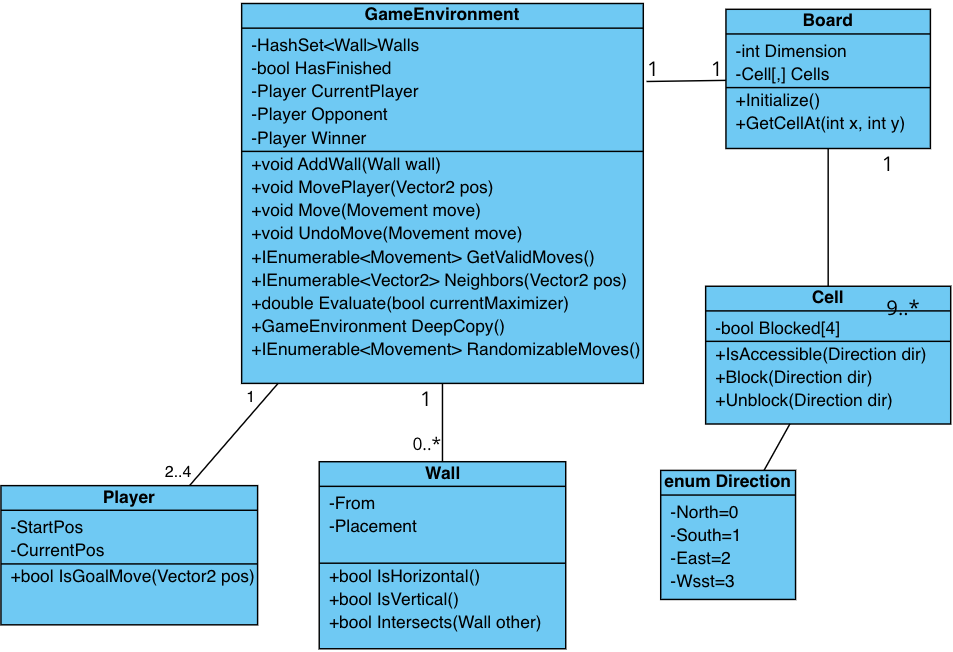
\includegraphics[width=.95\linewidth]{../img/uml_core.png}
    \caption{A UML diagram depicting relationship in the core library}
    \label{fig:core_uml}
\end{figure}

\subsection{Project Structure}

The solution consists of six fundamental projects, each written in \ac{Csharp}.

\begin{itemize}
    \item \textbf{Quoridor.Core}\\
        This library project contains the core game logic for Quoridor, and implements all interfaces to allow \ac{AI} algorithms to run.
        
    \item \textbf{Quoridor.AI}\\
        This library project includes all the fundamental interfaces and a generic \ac{AI} algorithms implemented using these interfaces.

    \item \textbf{Quoridor.Common}\\
        This library project includes all common helpers, such as XML parser helper, logging helper, etc.

    \item \textbf{Quoridor.Tests}\\
        This NUnit test project includes all unit tests for robust development.

    \item \textbf{Quoridor.ConsoleApp}\\
        A CLI tool that runs simulations and allows user to play against an opponent with a visual interface.

    \item \textbf{Quoridor.DesktopApp}\\
        A WinForms application that allows user to play against one another or against various \ac{AI}.
\end{itemize}

These projects are inter-connected by references. For example from figure \ref{fig:proj_dep}, \textbf{Quoridor.AI} is a standalone library that contains all the interfaces, which is referenced by all other projects.
All project dependency structures are depicted in figure \ref{fig:proj_dep}.

\begin{figure}[h]
    \centering
    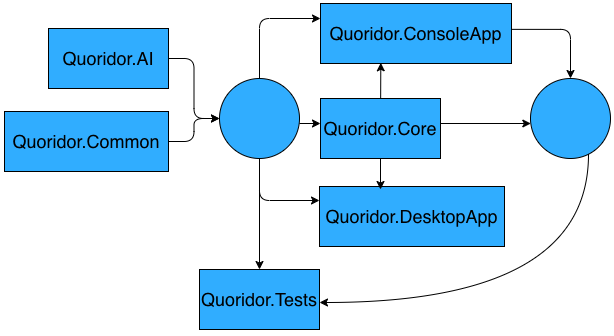
\includegraphics[width=.95\linewidth]{../img/project_structure.png}
    \caption{A project dependency diagram}
    \label{fig:proj_dep}
\end{figure}